%%
%% This is file `sample-manuscript.tex',
%% generated with the docstrip utility.
%%
%% The original source files were:
%%
%% samples.dtx  (with options: `manuscript')
%% 
%% IMPORTANT NOTICE:
%% 
%% For the copyright see the source file.
%% 
%% Any modified versions of this file must be renamed
%% with new filenames distinct from sample-manuscript.tex.
%% 
%% For distribution of the original source see the terms
%% for copying and modification in the file samples.dtx.
%% 
%% This generated file may be distributed as long as the
%% original source files, as listed above, are part of the
%% same distribution. (The sources need not necessarily be
%% in the same archive or directory.)
%%
%% The first command in your LaTeX source must be the \documentclass command.
\documentclass[manuscript,screen]{acmart}

%%
%% \BibTeX command to typeset BibTeX logo in the docs
\AtBeginDocument{%
  \providecommand\BibTeX{{%
    \normalfont B\kern-0.5em{\scshape i\kern-0.25em b}\kern-0.8em\TeX}}}

%% Rights management information.  This information is sent to you
%% when you complete the rights form.  These commands have SAMPLE
%% values in them; it is your responsibility as an author to replace
%% the commands and values with those provided to you when you
%% complete the rights form.
\setcopyright{acmcopyright}
\copyrightyear{2022}
\acmYear{2022}
%\acmDOI{10.1145/1122445.1122456}

%% These commands are for a PROCEEDINGS abstract or paper.
\acmConference [RecSys'22] 
{Seattle, WA USA}
{16th ACM Conference on Recommender Systems, Seattle, WA USA, Sept. 18 - 23, 2022}

\acmBooktitle{Computer Science 381: Recommender Systems Research}

\acmPrice{15.00}
\acmISBN{978-1-4503-XXXX-X/18/06}


%%
%% Submission ID.
%% Use this when submitting an article to a sponsored event. You'll
%% receive a unique submission ID from the organizers
%% of the event, and this ID should be used as the parameter to this command.
%%\acmSubmissionID{123-A56-BU3}

%%
%% The majority of ACM publications use numbered citations and
%% references.  The command \citestyle{authoryear} switches to the
%% "author year" style.
%%
%% If you are preparing content for an event
%% sponsored by ACM SIGGRAPH, you must use the "author year" style of
%% citations and references.
%% Uncommenting
%% the next command will enable that style.
%%\citestyle{acmauthoryear}

%%
%% end of the preamble, start of the body of the document source.
\begin{document}

%%
%% The "title" command has an optional parameter,
%% allowing the author to define a "short title" to be used in page headers.
\title{Evaluating the Accuracy and Coverage Performance of Collaborative Filtering, Content-based, and Hybrid Recommender Systems}

%%
%% The "author" command and its associated commands are used to define
%% the authors and their affiliations.
%% Of note is the shared affiliation of the first two authors, and the
%% "authornote" and "authornotemark" commands
%% used to denote shared contribution to the research.

\author{Brad Shook}
\affiliation{%
  \institution{Davidson College}
  \streetaddress{102 N Main Street}
  \city{ Davidson}
  \state{ North Carolina}
  \postcode{ 28035}
  \country{USA} }
\email{brshook@davidson.edu}

\author{Daniel Cowan}
\affiliation{%
  \institution{Davidson College}
  \streetaddress{102 N Main Street}
  \city{ Davidson}
  \state{ North Carolina}
  \postcode{ 28035}
    \country{USA} } 
\email{dacowandavidson.edu}

\author{Drew Dibble}
\affiliation{%
  \institution{Davidson College}
  \streetaddress{102 N Main Street}
  \city{ Davidson}
  \state{ North Carolina}
  \postcode{ 28035}
    \country{USA} } 
\email{drdibble@davidson.edu}

%%
%% By default, the full list of authors will be used in the page
%% headers. Often, this list is too long, and will overlap
%% other information printed in the page headers. This command allows
%% the author to define a more concise list
%% of authors' names for this purpose.
\renewcommand{\shortauthors}{NAMES: Brad Shook, Daniel Cowan, Drew Dibble}

%%
%% The abstract is a short summary of the work to be presented in the
%% article.
\begin{abstract}
Recommender systems provide users with personalized recommendations, saving users time in sifting through all of the available products and services on a given platform. Of course, there are many choices that can be made to develop the most accurate recommender system. This paper examines three types of recommender systems: collaborative filtering, content-based, and hybrid recommender systems, evaluating the performance of each system in terms of accuracy and coverage.
\end{abstract}

%%
%% The code below is generated by the tool at http://dl.acm.org/ccs.cfm.
%% Please copy and paste the code instead of the example below.
%%
%\begin{CCSXML}
%<ccs2012>
% <concept>
%  <concept_id>10010520.10010553.10010562</concept_id>
%  <concept_desc>Computer systems organization~Embedded systems</concept_desc>
%  <concept_significance>500</concept_significance>
% </concept>
% <concept>
%  <concept_id>10010520.10010575.10010755</concept_id>
%  <concept_desc>Computer systems organization~Redundancy</concept_desc>
%  <concept_significance>300</concept_significance>
% </concept>
% <concept>
%  <concept_id>10010520.10010553.10010554</concept_id>
%  <concept_desc>Computer systems organization~Robotics</concept_desc>
%  <concept_significance>100</concept_significance>
% </concept>
% <concept>
%  <concept_id>10003033.10003083.10003095</concept_id>
%  <concept_desc>Networks~Network reliability</concept_desc>
%  <concept_significance>100</concept_significance>
% </concept>
%</ccs2012>
%\end{CCSXML}
%
%\ccsdesc[500]{Computer systems organization~Embedded systems}
%\ccsdesc[300]{Computer systems organization~Redundancy}
%\ccsdesc{Computer systems organization~Robotics}
%\ccsdesc[100]{Networks~Network reliability}

%%
%% Keywords. The author(s) should pick words that accurately describe
%% the work being presented. Separate the keywords with commas.
\keywords{Recommender Systems, Collaborative Filtering, Content-based, Hybrid, Similarity and Prediction techniques}


%%
%% This command processes the author and affiliation and title
%% information and builds the first part of the formatted document.
\maketitle

\section{Introduction}
The continued shift towards online retail has left users with choices to make everywhere they look. This shift also allows companies to gather an immense amount of data on each user. Companies can track not only the user’s purchases, but all of their interactions with the company’s platform, including clicks, history, time spent on a page, etc. All of this data can be used to paint a complete picture of a user’s preferences and interests. Once a company gathers this data on the user’s preferences, recommender system harness the data to provide personalized recommendations to the user. These recommendations ease the burden on the user of sifting through all of their options while simultaneously increasing the companies likelihood of providing accurate recommendations to the user.

There are three overarching types of recommender systems: collaborative filtering (CF), content-based (CB), and hybrid (HYB) recommender systems. Collaborative filtering can be performed using a user-based method, an item-based method, through matrix factorization, or even through a neural network. A user-based collaborative filtering recommender system provides recommendations based on what other, similar users have enjoyed in the past. A user-based recommender system can struggle with scalability, the cold-start issue when there is little data, and sparsity, when only a small percentage of the available items are rated by users. In contrast, an item-based collaborative filtering recommender system provides recommendations similar to items that a user has liked in the past. Item-based recommender systems typically scale better than user-based recommender systems because the similarity between items is often more static than the similarity between users. However, item-based recommender systems similarly struggle with the cold-start issue and the issue of sparsity. Within both user-based and item-based collaborative filtering recommender systems, there are two primary choices for calculating similarity: Euclidean distance for recommender systems and Pearson correlation. Euclidean distance for recommender systems measures the linear distance between data points on an x, y plane to calculate similarity while Pearson correlation is a continuous measure (between -1 and 1) of how well two data points correlate.

Another example of collaborative filtering that we will examine is matrix factorization (MF). Like user-based and item-based collaborative filtering, matrix factorization uses data within a User-Item (U-I) matrix. However, it does not compute similarities between users and items. Instead, matrix factorization uses linear algebra to find two or more matrices that, when multiplied together, yield an approximation of the U-I matrix. Matrix factorization uses latent factors that help explain the interactions between users and items. An example of such a feature for a movie would be a specific genre or leading actor. To best approximate the U-I matrix, matrix factorization relies on algorithms such as stochastic gradient descent or alternating least squares to iteratively minimize the error between the predicted and actual ratings. Matrix factorization is much faster than item-based and user-based collaborative filtering, but the disadvantages are that it can be difficult to tune the hyperparameters and models can easily overfit or underfit the data. The final collaborative filtering model that we construct is based on a neural network. Like matrix factorization, this deep learning model uses a stochastic gradient descent optimizer. The model takes in both user and item information as vectors before passing them through a multi-layer neural architecture to calculate the predicted rating. \cite{Xiangnan2017}

We will also examine content-based methods, which utilize item descriptions and a profile of user interests. The specific content-based method we employ is the Term-Frequency-Inverse Document Frequency (TF-IDF) model. This model highlights the distinct words used in each item description by measuring how often each word appears in the descriptions before reducing the weight of common terms. The similarity between each item’s TF-IDF vector is then calculated using cosine similarity.

Finally, we will examine hybrid recommender systems, which combine components of collaborative filtering and content-based methods. Our hybrid approaches will begin with our TF-IDF model and replace values of the cosine similarity matrix using item-based similarities when the cosine similarity fails to meet given thresholds. The goal will be to limit the disadvantages of either method individually. \cite{Burke2002}


\section{Related Work}
There has been plenty of literature on collaborative filtering, content-based, and hybrid recommender systems. This previous literature informs our decision making through the development, experimentation, and evaluation of our recommender systems. Desrosiers and Karypis discuss neighborhood-based methods, He et al. discuss a neural network approach, Koren et al. discuss matrix factorization, Burke discusses hybrid techniques, Herlocker et al. discuss collaborative filtering and experimental design, and Seminario and Wilson introduce a key evaluation metric. The following paragraphs provide additional details about the findings in these papers and how they guide this report. 

Desrosiers and Karypis evaluate neighborhood-based methods, discussing the positives and negatives to both user-based and item-based recommender systems. The paper focuses on comparing the accuracy, efficiency, stability, justifiability, and serendipity of both methods. With accuracy, Desrosiers and Karypis note that it depends on the ratio of the number of items and users. In cases where the number of users is much greater than the number of items, item-based is likely to outperform user-based in terms of accuracy. In regards to efficiency, item-based methods are more scalable. The stability of each algorithm depends upon which of the two, users or items, is changing more often. If users are constantly updating, while items are relatively static, an item-based algorithm will be more stable. This is because the item-item similarity weights could be computed at infrequent time intervals if the items are relatively static. If the available items is constantly changing, while users are relatively static, a user-based algorithm will be more stable for the same reason. Item-based algorithms are more justifiable, as the user will be able to see that they are being recommended an item based on its similarity to an item they previously enjoyed. Finally, user-based recommender systems typically produce more serendipitous recommendations. This is because item-based recommender systems are likely to recommend items that are very similar to previously highly rated items by that user. In contrast, a user-based recommender system may recommend completely new items that were highly rated by a similar user. \cite{Desrosiers2011}


He et al. present a framework to construct a collaborative filtering model based on neural networks. The generalized framework as shown in Figure \ref{fig:framework} takes in user and item data as inputs and encodes both vectors using one-hot encoding before sending them through a multi-layer neural architecture to predict a score. Finally, the model is optimized using stochastic gradient descent. \cite{Xiangnan2017} We will utilize this generalized framework to construct our neural collaborative filtering recommender system. 

\begin{figure}[h]
  \centering
  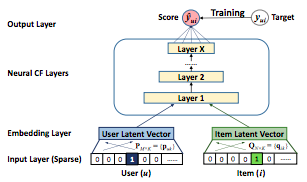
\includegraphics[width=0.65\textwidth]{figures/NCF_framework.png}
  \caption{Generalized NCF framework presented in He et al.'s \emph{Neural Collaborative Filtering}}
  \label{fig:framework}
\end{figure}

Koren et al. introduce matrix factorization as a recommender system technique, finding that it has the potential to be both scalable and accurate. They discuss how matrix factorization offers advantages in its ability to utilize implicit feedback from a user. Rather than an explicit rating of an item, implicit data might be time spent on site, browser history, mouse movements, etc. They also identify stochastic gradient descent and alternating least squares as two primary learning algorithms for matrix factorization models. 

Burke introduces many hybridization techniques that have been experimented with and employed as recommender systems. The paper notes that hybridization techniques have the ability to outperform any one method on its own. The paper specifically outlines seven hybridization techniques, discussing the positives and negatives of each. \cite{Burke2002}

Herlocker et al. break down the collaborative filtering process into its component parts and provides additional ways of improving a collaborative-based recommendation system. They dive into the various similarity functions, remarking that the performance of similarity functions depends upon the rating scale. They also find that significance weighting can improve accuracy by limiting the effect of neighbors that appear highly similar but only share a few rated items. We will utilize their experimental design to identify the best parameters in our recommender systems.\cite{Herlocker1999}

Finally, Seminario and Wilson developed a straightforward "AC Measure" used to evaluate the accuracy and coverage of a recommender system. The measure is calculated as follows: 
$
AC_i = \frac{Accuracy_i}{Coverage_i}
$
where $i$ represents the $i$th trial in an experiment. We will not use the AC Measure due to some of our models producing coverages of 100\% despite changes in hyperparameter sets. This issue is discussed further in our Thesis and Discussion sections. With that being said, this metric highlights the importance of balancing the trade-off between accuracy and coverage when evaluating recommender systems.  \cite{Seminario2012}

\section{Thesis}
In this paper, we will compare the performance, in terms of accuracy and coverage, of the following 10 recommender systems: 1) user-based collaborative filtering using Euclidean distance for user-user similarity calculations (UU-CF-D), 2) user-based collaborative filtering using Pearson similarity (UU-CF-P), 3) item-based collaborative filtering using Euclidean distance (II-CF-D), 4) item-based collaborative filtering using Pearson similarity (II-CF-P), 5) matrix factorization collaborative filtering with stochastic gradient descent (MF-SGD), 6) matrix factorization collaborative filtering with alternating least squares (MF-ALS), 7) TFIDF content-based method with cosine similarity for content similarity calculations (TFIDF), 8) a hybrid model using a combination of the II-CF-D and TFIDF methods (HYB-D), 9) a hybrid model using a combination of the II-CF-P and TFIDF methods (HYB-P), 10) and a neural collaborative filtering model (NCF). Note that we will compare each of these recommender systems’ performances against each other only after they have each been tuned to find the “best” set of hyperparameters for each recommender system.

The two distance measures to be tested on neighborhood-based user and item collaborative filtering models, as previously noted, are Euclidean distance and Pearson similarity. Euclidean calculates the simple straight-line distance between two points in space: \[  d\left( x,y\right)   = \sqrt {\sum _{i=1}^{n}  \left( x_{i}-y_{i}\right)^2 }\]

There are several intricacies that Euclidean distance cannot take into account when it is used to calculate the difference between users or items. For example, Euclidean distance cannot take into account correlations between users; the grade inflation issue is a good example of this. One user might only rate items between 2-4, while another might only rate items between 3-5. Pearson similarity solves this issue by measuring correlations between users or items rather than pure sameness. The formula is as follows: \[  P(x,y) = \frac{ \sum_{i=1}^{n}(x_i-\bar{x})(y_i-\bar{y}) }{%
        \sqrt{\sum_{i=1}^{n}(x_i-\bar{x})^2}\sqrt{\sum_{i=1}^{n}(y_i-\bar{y})^2}} \] The result of this distance ranges from -1 to 1 where 1 is most similar and -1 is most dissimilar.

As previously noted, the recommender systems’ performances will be compared against each other only after they have each been tuned to find the “best” set of hyperparameters. For the user- and item-based collaborative filtering models, the parameters tested were similarity threshold, the minimum similarity users or items must have to be considered in predicted ratings calculations, and significance weighting cut-off, a correction which gives higher weighting to users or items with a larger amount of users or items that are similar to it. The details of these parameters are further discussed in \cite{midterm}. Similarity threshold was the sole parameter searched for the TFIDF model. For the hybrid models, which combined the item-based and TFIDF approaches, we tuned both the similarity threshold and the weighting factor. In our hybrid model, the weighting factor represents the weight attached to an item-item similarity value when updating a value in the cosine similarity matrix from the TFIDF model. For the two matrix factorization models, we explored different values of the number of factors in the model, the value of the regularization term, and - in the case of MF-SGD - the value of the learning rate. Further explanation of these parameters can be found in \cite{last_asg}. For the NCF, we explored the number of hidden layers, number of factors, and the learning rate. We employed a grid search to tune these hyperparameters as discussed further in the Experimental Design. 

In order to determine the best parameter set for each model, we only considered the MSEs of models with at least 90\% coverage. Given that, among all models with their ideal parameter sets, we believe that a hybrid model will perform best, as studies have shown that combining the effects of collaborative filtering and content-based methods can improve a model's recommendations \cite{Burke2002}.

\section{Experimental Design}
To test the performance of each recommender system, we will use the ML-100k dataset from GroupLens.org. \footnote{\url{https://grouplens.org/datasets/movielens/100k/}} This dataset includes 100,000 ratings, on a scale of 1-5, from 943 users on 1682 movies. We will evaluate the performance of each model using either a train-test split or leave one out cross-validation (LOOCV). This approach measures the performance of a model by removing a specific value from the dataset, using the remainder of the dataset to predict that missing value, and then comparing the actual and predicted values. We will primarily rely upon computed mean squared error (MSE) for our evaluation while requiring that the models yield a coverage of greater than 90\%. In Tables \ref{fig:mostrated}, \ref{fig:highestrated},  and \ref{fig:mostwithhighest}, along with Figure \ref{hist}, we summarize the dataset used in this experiment. Take note that we are working with a dataset that is heavily right-skewed, with most of the ratings being > 3.

\begin{table}
\[\begin{array}{c|c}
\text{Statistic} & \text{Value}\\
\hline
\text{Number of users} & 943\\
\text{Number of items} & 1664\\
\text{Number of ratings} & 99693\\
\text{Overall average rating (std. dev.)} & 3.53 (1.13)\\
\text{Average item rating (std. dev.)} & 3.08 (0.78)\\
\text{Average user rating (std. dev.)} & 3.59 (0.44)\\
\text{Average ratings per user (std. dev.)} & 105.72 (100.57)\\
\text{Min. \# of ratings for single user} & 19\\
\text{Max. \# of ratings for single user} & 736\\
\text{Median \# of ratings for single user} & 64\\
\text{Matrix sparsity} & 93.65\%\\
\end{array}\]
\caption{General statistics describing the dataset used in the experiment.}
\label{fig:stats}
\end{table}


\begin{table}[]
\begin{tabular}{l|l}
\text{Movie} & \text{Number of Ratings}\\
\hline
Star Wars (1977)          & 583 \\
Contact (1997)            & 509 \\
Fargo (1996)              & 508 \\
Return of the Jedi (1983) & 507 \\
Liar Liar (1997)          & 485
\end{tabular}
\caption{The most rated movies in the dataset.}
\label{fig:mostrated}
\end{table}

\begin{table}[]
\begin{tabular}{l|l}
\text{Movie} & \text{Average Rating}\\
\hline
Saint of Fort Washington, The (1993) & 5.0 \\
Prefontaine (1997)                   & 5.0 \\
Great Day in Harlem, A (1994)        & 5.0 \\
They Made Me a Criminal (1939)       & 5.0 \\
Santa with Muscles (1996)            & 5.0
\end{tabular}
\caption{The highest rated movies in the dataset.}
\label{fig:highestrated}
\end{table}

\begin{table}[]
\begin{tabular}{l|l|l}
\text{Movie} & \text{Average Rating} & \text{Number of Ratings}\\
\hline
Close Shave, A (1995)            & 4.49 & 112 \\
Schindler's List (1993)          & 4.47 & 298 \\
Wrong Trousers, The (1993)       & 4.47 & 118 \\
Casablanca (1942)                & 4.46 & 243 \\
Shawshank Redemption, The (1994) & 4.45 & 283
\end{tabular}
\caption{The highest rated movies in the dataset with at least 100 ratings.}
\label{fig:mostwithhighest}
\end{table}

\begin{figure}[h]
  \centering
  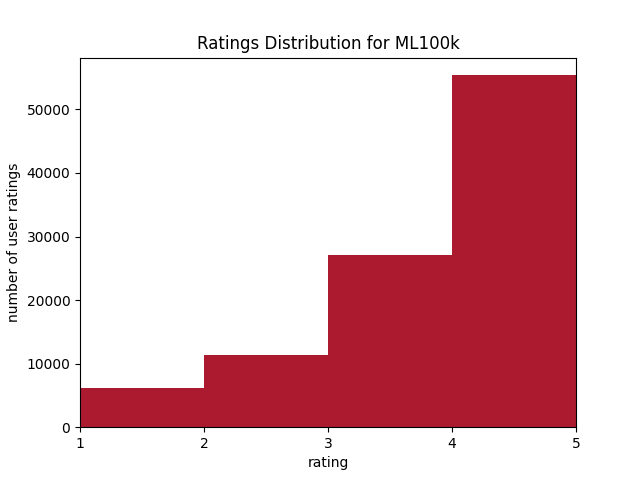
\includegraphics[width=0.65\textwidth]{ratings_hist.png}
  \caption{Histogram of the ratings in the dataset.}
  \label{hist}
\end{figure}

In order to determine which of the 10 models evaluated in this experiment make the most accurate recommendations, the ideal parameter sets for each model must be identified so that we are confident that we are comparing the best models within each framework. For each model, a grid search was used to search the parameter space, and the accuracy and coverage for each model was recorded. The best-performing set of parameters for each model was chosen to be used in the final evaluation. Of note, only models where coverage (where applicable) was greater than 90\% were considered to be candidates for best model.

For the user- and item-based recommenders (UU-CF-D, UU-CF-P, II-CF-D, II-CF-P), the details of the grid search as well as the parameter space that was explored are explained in \cite{midterm}. These grid searches found UU-CF-D performed best with a similarity threshold of 0.1 and similarity significance weighting of 25 while the UU-CF-P employed a threshold of 0.3 and a weighting of 25. Additionally, the best-performing item-based recommenders utilized a similarity threshold of 0.0 and a similarity significance weighting of 100. 

The same details for the matrix factorization models (MF-SGD, MF-ALS) are discussed in \cite{last_asg}. It was determined that MF-SGD yielded the best MSE when 200 factors, a learning rate of 0.02, and a beta regularization term of 0.02 were used. As for the MF-ALS, the best parameter set was 2 factors and a regularization term of 0.1. It should be noted that the accuracy of the MF models was evaluated on a holdout test dataset of 20\%.

For TFIDF, we searched over a single hyperparameter: similarity threshold. The similarity threshold determines the range of values to be considered in the cosine similarity matrix. For example, if the similarity threshold is 0.5, then only cosine similarities greater than 0.5 will be considered when generating predictions and recommendations. In order to determine what similarity threshold values to search over, we calculated the mean and standard deviation of the cosine similarity matrix, while ensuring no duplicate item-item combinations were used in the calculations. The mean of these similarities was 0.577 and the standard deviation was 0.27. These values led us to use the similarity threshold values of 0, 0.306, 0.577, and 0.847, which include the mean and the mean plus/minus the standard deviation. LOOCV was used to determine the accuracy of the model. 
    
As for the Hybrid models, their grid search searched over two hyperparameters: similarity threshold and weighting factor. The similarity thresholds were the same that were used in TFIDF. For the weighting factors, we searched over the values of 0.25, 0.5, 0.75, and 1. Like TFIDF, LOOCV evaluated the performance of the model.

The NCF was tuned using a grid search of three hyperparameters: number of hidden layers, number of factors, and learning rate. The number of layers in the model ranged from 10 to 6, with each following layer decreasing in number of nodes by a power of 2 (ie. 256,128,64,32,16,8,4,2). The factors are equivalent to those used in matrix factorization. Specifically, the user and item inputs are mapped to a latent factor vector, whose dimension is determined by the number of factors, then fed into the neural network. Lastly, the grid search included the following learning rates: 1e-1, 1e-2, 1e-3, 1e-4. It is important for neural networks to use a learning rate that ensures the model learns "smoothly", meaning the loss does not make huge leaps. Moreover, we appended a dropout layer followed by a batch normalization layer to each hidden layer. Dropout layers are used to reduce overfitting in neural networks \cite{Hinton2012} while batch normalization reduces the possibility of vanishing gradients during training \cite{Ioffe2015}. For each model in the grid search, early stopping was used. Early stopping involves monitoring the validation loss metric after each epoch. If the metric does not improve for a certain number of epochs (a.k.a patience), then the model stops training. For our implementation, we used a patience of 5 and an upper bound of 250 epochs, meaning each model would stop training early or end at epoch 250. By implementing early stopping, we ensure each model, invariant of the learning rate and architecture, is able to converge in terms of validation loss. Lastly, a train-validation-test split of 80\%-10\%-10\% was used. Therefore, each model was evaluated on 10\% of the dataset instead of the whole dataset.

After determining the best parameter sets for each of the 10 models, we set out to compare them to one another. To do so, we compared the mean squared error and coverage of each of the models, after which we explored possible reasons for these differences and whether they matched our original hypothesis. We also used z-tests (we decided against the standard t-test because our sample sizes are larger) and ANOVA to ensure that the means of the errors associated with each model were statistically different from each other.


\section{Results}

\subsection{Grid Searches}

For the TFIDF algorithm, we found that the model which had the highest coverage and lowest MSE had a similarity threshold of 0. The MSE and coverage that this model yielded was 1.048402 and 0.99743, respectively. Both coverage and MSE worsened as the similarity thresholds increased, as shown in Figure \ref{tfidf_grid}. It was expected that coverage would worsen as the similarity threshold increased, but it was interesting to find that MSE did as well. We would generally expect that a higher similarity threshold would result in lower coverage but a lower MSE, so this was an intriguing development. 

\begin{figure}[h]
  \centering
  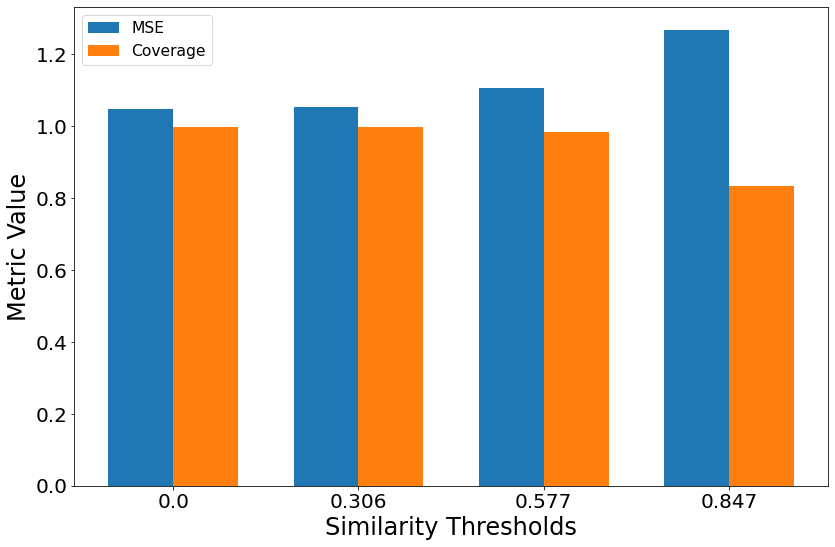
\includegraphics[width=0.6\textwidth]{figures/tfidf_grid_results.png}
  \caption{MSEs and coverage results from the TFIDF grid search. }
  \Description{MSEs and coverage results from the TFIDF grid search. }
  \label{tfidf_grid}
\end{figure}

Through our hybrid grid searches, whose results are shown in Figure \ref{hyb_mse_vs_weighting_factor}, the HYB-D model that yielded the lowest MSE had a similarity threshold of 0 and a weighting factor of 1. Like the HYB-D model, the best performing HYB-P model used the same hyperparameters. These two models had MSEs of 1.001539 and 1.0296574, respectively, along with coverages of 0.99955 and 0.99930. Our analysis of this grid search found that similarity thresholds of 0.576448 and 0.846703 yielded the same evaluation statistics, invariant of the weighting factor. This was due to the similarity thresholds resulting in the same similarities being used to produce predictions each time. Moreover, we discovered a higher weighting factor generally resulted in models with lower MSEs. 

\begin{figure}[h]
  \centering
  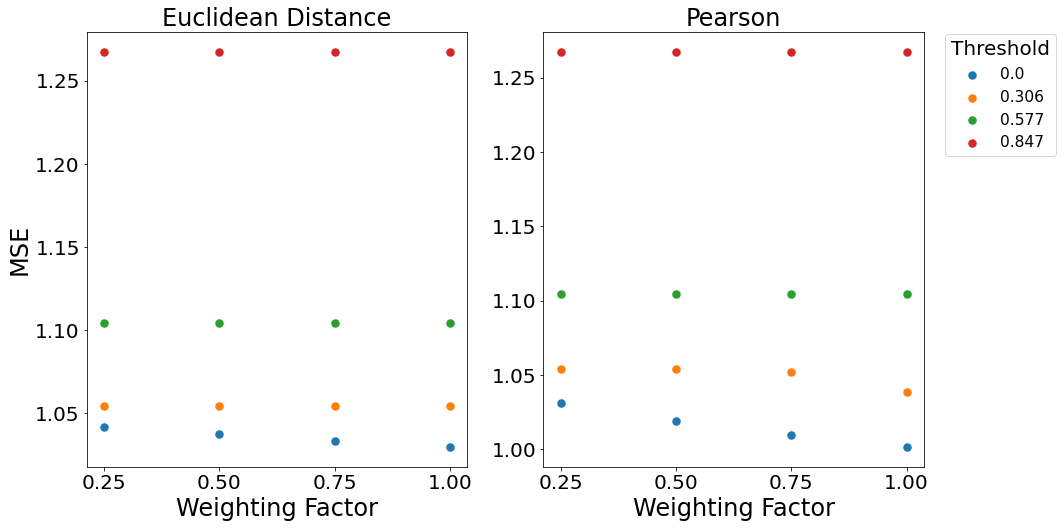
\includegraphics[width=0.8\textwidth]{figures/hyb_mse_vs_weighting_factor.png}
  \caption{MSE vs. weighting factor for HYB-D and HYB-P. }
  \Description{MSE vs. weighting factor for HYB-D and HYB-P. }
  \label{hyb_mse_vs_weighting_factor}
\end{figure}

After performing the grid search on the NCF, we identified the best performing model to be one that had a learning rate of 0.01, 100 factors, and an architecture with hidden dense layers with the following number of nodes: [64, 32, 16, 8, 4, 2, 1]. This model yielded a test MSE of 0.876653. Further analysis demonstrated that there were not any general trends among different values of the number of factors nor the learning rate, which can be seen in Figure \ref{mse_vs_factors_and_lr}. This was expected, at least for the learning rate, because the learning rates chosen are small enough to ensure smooth learning and early stopping ensures each model converges. However, it is fascinating that there were no specific trends among the number of factors since this parameter determines a whole layer in the neural network. 

\begin{figure}[h]
  \centering
  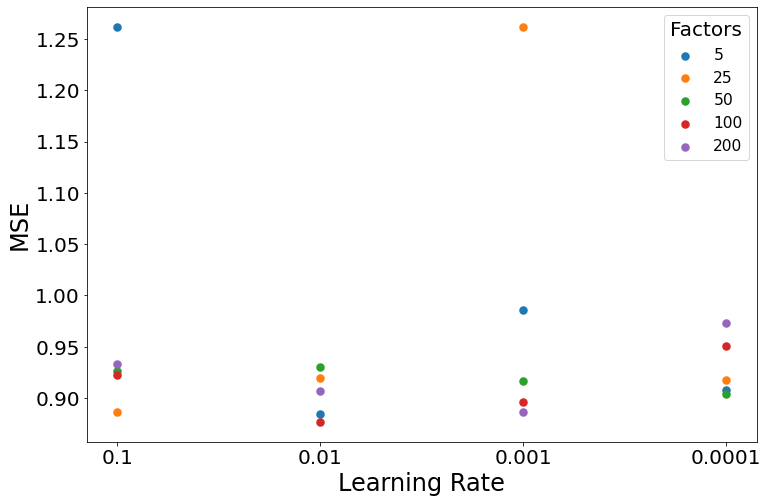
\includegraphics[width=0.6\textwidth]{figures/ncf_mse_vs_factors_and_lr.png}
  \caption{Scatter plot showing how the learning rate and number of factors affect the MSE when the following number of nodes are used: [64, 32, 16, 8, 4, 2, 1]. }
  \Description{Scatter plot showing how the learning rate and number of factors affect the MSE when the following number of nodes are used: [64, 32, 16, 8, 4, 2, 1]. }
  \label{mse_vs_factors_and_lr}
\end{figure}

\subsection{Model Comparison}

Using the best-performing models, we are able to compare the 10 models' performances versus one another. In Figure \ref{model_comparison}, we see the MSEs for each of these models. The figure shows that the model with the lowest MSE is II-CF-D. We see that every collaborative filtering model had a lower MSE than the content-based and hybrid models. Another observation is that TFIDF had the highest MSE out of all the models. We can also derive that the HYB models were able to successfully combine both TFIDF and II-CF because the HYB coverages are higher than the II-CF models and the HYB MSEs are lower than the TFIDF model. Moreover, differing similarity methods (Pearson and Euclidean distance) had a minimal effect on the MSE of the models.

\begin{figure}[h]
  \centering
  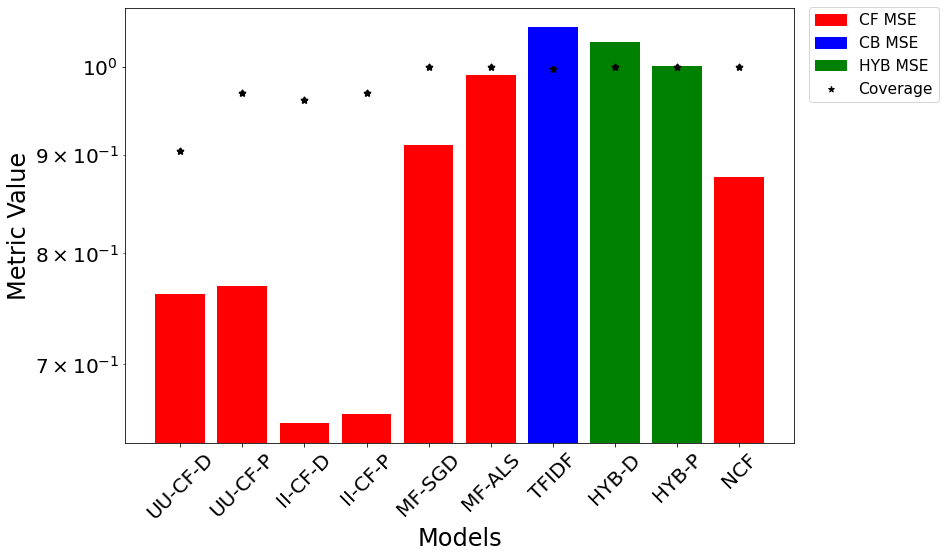
\includegraphics[width=0.6\textwidth]{figures/model_comparison_bar.png}
  \caption{MSE vs. weighting factor for HYB-D and HYB-P. }
  \Description{MSE vs. weighting factor for HYB-D and HYB-P. }
  \label{model_comparison}
\end{figure}

Another important factor to consider when comparing these models is the coverage. Though II-CF-D, II-CF-P, UU-CF-D, and UU-CF-P had the lowest MSEs, they also had the lowest coverage. The other 6 models all had coverages greater than 99.7\%. 

Also of note, an ANOVA test confirmed that these sample means are statistically different from each other, and several two-sample z-tests revealed that each of these models produce errors that are statistically and significantly different from each other, indicating that the MSEs of each of these models are reliably different from each other and are not the result of chance.

\section{Discussion}
The model comparison shows that our hypothesis was not true since the models with the lowest MSEs were collaborative filtering models. Moreover, even if we take into account coverage, then the MF-SGD, MF-ALS, and NCF models still outperform the hybrid models. Though the NCF and MF models yielded the lowest MSEs and highest coverage combinations, we cannot make a concrete statement about these models when comparing them to the other seven. This is due to the evaluation method used with these models. As mentioned previously, the MF models were trained on 80\% of the dataset and then evaluated on 20\%. Similarly, the NCF was trained on 80\% of the dataset and evaluated on 10\%. In contrast to this, the other seven models were evaluated on the whole dataset during LOOCV, ensuring that the MSE represents the true performance of the models. Since the MF and NCF models are trained on 80\% of the dataset, it does not make sense to evaluate their performance on the whole dataset since it would be biased. However, only using the test splits for evaluation may not provide the true performance of the models. Therefore, these models are not directly comparable. 


\section{Conclusion}
% Summary of the work completed and the findings that were made. Future work is also included in this section.

In this work, we compared 10 tuned recommender algorithms. Through our analysis, we determined that collaborative filtering algorithms yielded lower MSEs but also lower coverages than content-based and hybrid models. In addition, we found that the MF and NCF models provided low MSEs while maintaining high coverage. Despite this, we recommend further testing and evaluations of these models. Concretely, we suggest deploying k-fold cross validation, which would allow for the true performance of the MF and NCF models to be determined. Furthermore, another variation to the NCF that could be tested is using one-hot encoding for the user and item inputs. This could allow the model to more easily learn since it would take as input only 1s and 0s. Lastly, He et al. proprosed a neural matrix factorization model in \cite{Xiangnan2017} which is an extension of the NCF implemented in this paper. Such a model could provide better results than the simple NCF mentioned here. 

\newpage

%%
%% The next two lines define the bibliography style to be used, and
%% the bibliography file.
\bibliographystyle{ACM-Reference-Format}
\bibliography{sample-base}





\bigskip























\end{document}
\endinput
%%
%% End of file `sample-manuscript.tex'.
